% vim:set et fenc=utf-8 ft=tex sw=2 ts=2 tw=72:

\newif\ifdraft
% \drafttrue

\ifdraft
        \documentclass[conference, draftclsnofoot, draft]{IEEEtran}
        \def\baselinestretch{1}
        \setlength{\marginparwidth}{2cm}
\else
        \documentclass[conference]{IEEEtran}
\fi

\usepackage[T1]{fontenc}
\usepackage[utf8]{inputenc}

\usepackage[hyphens]{url} \urlstyle{same}

%% Citations
\usepackage[nospace]{cite}

%% Table Support
\usepackage{dcolumn}
\usepackage{longtable}
\usepackage{multirow}
\usepackage{booktabs}
\usepackage{tabulary}

%% Extra support
\usepackage{xspace}
\usepackage{amsmath}
\usepackage{algorithm}
\usepackage{balance}
\usepackage{placeins}

%% Algorithms
\usepackage{algorithm}
\usepackage{algpseudocode}

%% Graphics
\usepackage{tikz}
\usepackage{pgfplots}
\usepackage{pgfplotstable}
\usepackage{xcolor}
\usepackage{color}
\usepackage{listings}

%% Tikz
\usetikzlibrary{positioning, arrows}

% Chart Colors
\definecolor{chartblue}{HTML}{3366CC}
\definecolor{chartred}{HTML}{DC3912}
\definecolor{chartyellow}{HTML}{FF9900}
\definecolor{chartgreen}{HTML}{109618}
\definecolor{chartmagenta}{HTML}{990099}
\definecolor{chartpurple}{HTML}{3B3EAC}

% \ifdraft
%     \usepackage[colorinlistoftodos]{todonotes}
%     \newcommand{\evan}[1]{{\color{blue}\emph{Evan Says: #1}}\xspace}
%     \newcommand{\evantodo}[1]{{\color{blue}\emph{Evan Todo: #1}}\xspace}
%     \newcommand{\dmg}[1]{{\color{blue}\emph{dmg Says: #1}}\xspace}
%     \newcommand{\dmgtodo}[1]{{\color{blue}\emph{dmg Todo: #1}}\xspace}
% \else
%     \usepackage[disable]{todonotes}
%     \newcommand{\evan}[1]{}
%     \newcommand{\evantodo}[1]{}
%     \newcommand{\dmg}[1]{}
%     \newcommand{\dmgtodo}[1]{}
% \fi
    \usepackage[colorinlistoftodos]{todonotes}

\newcommand{\tool}{{\emph Linvis}\xspace}


    \newcommand{\evan}[1]{{\color{blue}\emph{Evan Says: #1}}\xspace}
    \newcommand{\evantodo}[1]{{\color{blue}\emph{Evan Todo: #1}}\xspace}
    \newcommand{\dmg}[1]{{\color{blue}\emph{dmg Says: #1}}\xspace}
    \newcommand{\dmgtodo}[1]{{\color{blue}\emph{dmg Todo: #1}}\xspace}


%%% Local Variables:
%%% mode: plain-tex
%%% TeX-master: t
%%% End:


\newcommand{\TheTitle}{Merge-Tree: Visualizing the Integration of Commits into Linux}
\newcommand{\TheAuthors}{Evan Wilde, Daniel M. German}
\newcommand{\TheEmails}{etcwilde@uvic.ca, dmg@uvic.ca}
\newcommand{\TheSubject}{Understanding a large number of commits and merges}
\newcommand{\TheKeywords}{Linux, git, visualizations}

%% Referencing
\usepackage[unicode=true,
          pdftitle={\TheTitle},
          pdfauthor={\TheAuthors},
          colorlinks=false]{hyperref}

\lstset{frame=tb,
  language=python,
  aboveskip=3mm,
  belowskip=3mm,
  showstringspaces=false,
  columns=flexible,
  basicstyle={\small\ttfamily},
  numbers=none,
  numberstyle=\tiny\color{gray},
  keywordstyle=\color{chartblue},
  commentstyle=\color{chartred},
  stringstyle=\color{chartgreen},
  breaklines=true,
  breakatwhitespace=true,
  tabsize=3
}

\synctex=1

\begin{document}

\title{\TheTitle}

\author{
        \IEEEauthorblockA{\TheAuthors}
        \IEEEauthorblockN{Department of Computer Science,
                University of Victoria, Canada.}
        \IEEEauthorblockA{Email: \TheEmails}
}
\maketitle

\begin{abstract}
\end{abstract}

\begin{IEEEkeywords}
  \TheKeywords
\end{IEEEkeywords}

\section{Introduction}
\label{sec:introduction}

Git is a distributed version control system that is used in many
open-source and closed-source projects. Git enables many developers to
write code simultaneously, working on various components known as
branches. Git uses a directed acyclic graph model (DAG) for storing the
necessary information regarding the state of the code at any point in
time. Git refers to nodes of the DAG as commits, not distinguishing
between the code-carrying commits and the structural commits that bring
two branches together. In this paper, we will refer to the individual
commits as being commits, the structural merge commits as merges, and
refereeing to all as repository events.

Between 50k and 70k commits are added to the Linux kernel per version
requiring maintainers of older versions of the kernel to sift through
thousands of commits and merges with tools that are unable to filter and
effectively visualize projects at the scale of the kernel. Older
versions of the kernel are used in embedded systems and mobile phones;
for security purposes, performance needs, and changing hardware
requirements, maintainers must be able to understand the changes being
made in the current version of the kernel in order to produce the
necessary patches for the older versions of the kernel. Current tools
and visualizations are based on the directed acyclic graph (DAG) of the
repository, showing all commits and merges in chronological order by
when the commit was authored, not by when it arrived in the official
Linux repository.

\begin{figure}
  \centering
  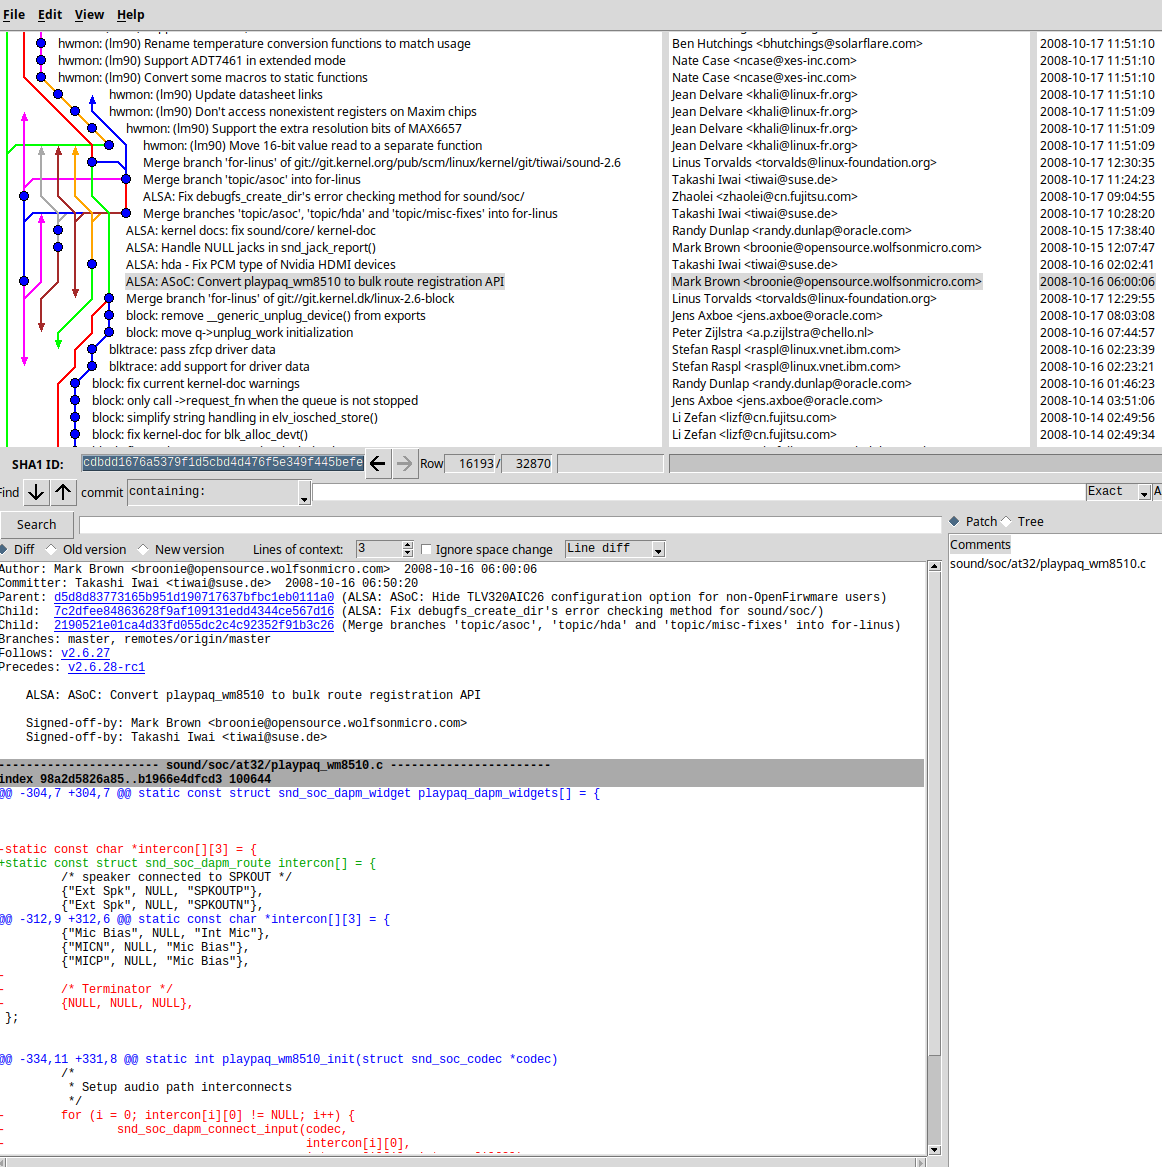
\includegraphics[width=0.8\linewidth]{figures/gitk.png}
  \caption{
    The Gitk interface, centered at commit
    cdbdd1676a5379f1d5cbd4d476f5e349f445befe. The top left pane showing
    the DAG, the top center pane showing the authors, and top right pane
    showing the commit dates. The bottom-left pane shows the full
    commit message and diff of the selected commit, and the bottom-right
    pane shows the list of the files modified by the selected commit.
  }
  \label{fig:gitk}
  %\vspace{-4mm}
\end{figure}

% DAG model

The DAG representation works in smaller projects; it enables users to
see when changes are made, when these changes are merged, how each
branch is interacting, and the point where a branch forks from the
master branch. In large modular projects, like the Linux kernel, the DAG
becomes a mess of merges and commits (Figure~\ref{fig:gitk}) losing its
visual meaning. In some cases, the repository is simply too large for
systems to generate a visualization; repositories stored on GitHub will
have a DAG visualization to show the branches and forks of a
repository, but is unable to display the visualization for projects at
the scale of Linux or even the Git Git
repository(Figure~\ref{fig:gitfail}). Between 60k and 70k new commits
are created for the Linux project every year; according to previous
work\cite{German2015}, a commit takes a median of 30 days from the time
it is authored until it arrives in the official repository. The snapshot
of the kernel tomorrow may be different than the snapshot from today,
containing new commits authored in the past; distinguishing these new
commits from the commits in the snapshot from today is not trivial.

\begin{figure}
  \centering
  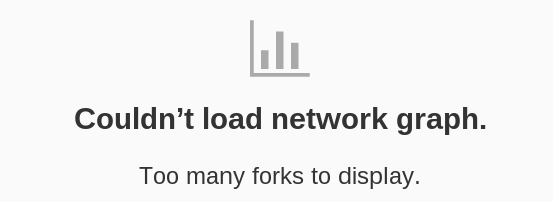
\includegraphics[width=0.8\linewidth]{figures/github_viewer.png}
  \caption{Github is unable to display the DAG of the Linux
    Project due to the size and complexity, which would normally
    show the relationship to other branches and forks.}
  \label{fig:gitfail}
  %\vspace{-2mm}
\end{figure}

% Merge tree model

We propose a new model, built from the DAG, with the purpose of
providing a clearer conceptual image of how a commit is merged, other
commits that are merged with a commit, and a summarization of the entire
group of commits that are merged with a commit. We call our model the
\mt model. The model inverts the DAG, so that reference point from
parent to child instead of from child to parent. This enables the
aggregation of commit metrics at merges. Given a merge, we are able to
recursively traverse the children of the merge, collecting the
statistics at each commit. The commits become the leaves of the tree,
and internal nodes are merges that do not merge into the master branch
of the repository. We terminate the further traversal of an edge under
two conditions; first, if the next event is on the master branch of the
repository, second, if the next event has a shorter path into the master
branch of the repository. As a consequence, commits will always take the
shortest path, in terms of commit time, to the master branch.

A short example: assume the commits represented in
Figure~\ref{fig:repoEvents} show the sequence of events in a repository.
In this case, commits are performed in various repositories and
branches. The DAG representation of the commits is shown in
Figure~\ref{fig:repoDAG}. Notice that the DAG loses information about
the master branch and the repository that the master branch is part of.
The \mt view of this DAG is visible in Figure~\ref{fig:repoTree}.
Note that the direction of the edges of the DAG have been inverted,
instead of pointing from the child to the ancestors, it points from the
ancestor to its successors, forming a path to the master branch. Also
note that the DAG has been simplified, showing only a single edge on the
path to master for any commit.

\begin{figure}[htbp]
  \centering
  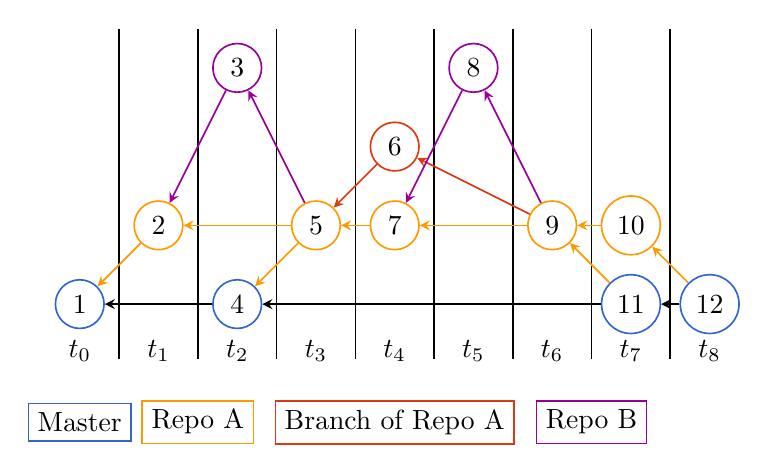
\begin{tikzpicture}[auto, on grid, semithick, state/.style={circle, text=black}]
    \foreach \x in {0, 1, 2, 3, 4, 5, 6, 7}
    \draw[shift={(\x + 0.5, -0.5)}, color=black] (0cm, 4cm) -- (0pt, -0.2cm);

    \node[state, draw=chartblue] (1) {1};
    \node[state, draw=chartyellow, above right= of 1] (2) {2};
    \node[state, draw=chartmagenta, above right= 2cm and 1cm of 2] (3) {3};
    \node[state, draw=chartblue, right= 2cm of 1] (4) {4};
    \node[state, draw=chartyellow, above right=of 4] (5) {5};
    \node[state, draw=chartred, above right=of 5] (6) {6};
    \node[state, draw=chartyellow, right=of 5] (7) {7};
    \node[state, draw=chartmagenta, above right= 2cm and 1cm of 7](8) {8};
    \node[state, draw=chartyellow, right= 2cm of 7] (9) {9};
    \node[state, draw=chartyellow, right=of 9] (10) {10};
    \node[state, draw=chartblue, below right=of 9] (11) {11};
    \node[state, draw=chartblue, below right=of 10] (12) {12};

    \draw (12) edge[-stealth] (11) edge[chartyellow, -stealth] (10);
    \draw (11) edge[-stealth] (4) edge[chartyellow, -stealth] (9);
    \draw (10) edge[chartyellow, -stealth] (9);
    \draw (9) edge[chartmagenta, -stealth] (8) edge[chartred, -stealth] (6)
              edge[chartyellow, -stealth] (7);
    \draw (8) edge[chartmagenta, -stealth] (7);
    \draw (7) edge[chartyellow, -stealth] (5);
    \draw (6) edge[chartred, -stealth] (5);
    \draw (5) edge[chartmagenta, -stealth] (3) edge[chartyellow,-stealth] (2)
              edge[chartyellow, -stealth] (4);
    \draw (4) edge[-stealth] (1);
    \draw (3) edge[chartmagenta, -stealth] (2);
    \draw (2) edge[chartyellow, -stealth] (1);

    \node [draw=chartblue, below = 1.5cm of 1] (l1) {Master};
    \node [draw=chartyellow, right = 1.5cm of l1] (l2) {Repo A};
    \node [draw=chartred, right = 2.5cm of l2] (l3) {Branch of Repo A};
    \node [draw=chartmagenta, right= 2.5cm of l3] (l4) {Repo B};

        \foreach \x in {0, 1, 2, 3, 4, 5, 6, 7, 8}
    \node[shift={(\x, -0.6)}, color=black] {$t_\x$};
  \end{tikzpicture}
  \caption{Example of a sequence of events performed in different
    repositories. The horizontal axis represents time. Each horizontal
    section represents a different branch and/or repository. Each commit
    points to its ancestor.}
  \label{fig:repoEvents}
%\vspace{-3mm}
\end{figure}

\begin{figure}[htbp]
  \centering
  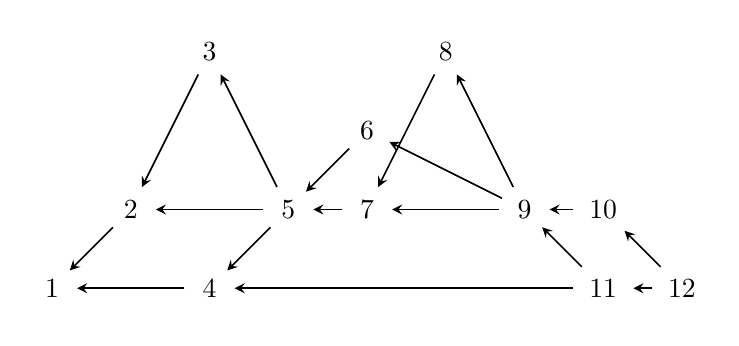
\begin{tikzpicture}[auto, on grid, semithick, state/.style={circle, text=black}]
    \node[state] (1) {1};
    \node[state, above right= of 1] (2) {2};
    \node[state, above right= 2cm and 1cm of 2] (3) {3};
    \node[state, right= 2cm of 1] (4) {4};
    \node[state, above right=of 4] (5) {5};
    \node[state, above right=of 5] (6) {6};
    \node[state, right=of 5] (7) {7};
    \node[state, above right= 2cm and 1cm of 7](8) {8};
    \node[state, right= 2cm of 7] (9) {9};
    \node[state, right=of 9] (10) {10};
    \node[state, below right=of 9] (11) {11};
    \node[state, below right=of 10] (12) {12};

    \draw (12) edge[-stealth] (11) edge[-stealth] (10);
    \draw (11) edge[-stealth] (4) edge[-stealth] (9);
    \draw (10) edge[-stealth] (9);
    \draw (9) edge[-stealth] (8) edge[-stealth] (6)
              edge[-stealth] (7);
    \draw (8) edge[-stealth] (7);
    \draw (7) edge[-stealth] (5);
    \draw (6) edge[-stealth] (5);
    \draw (5) edge[-stealth] (3) edge[-stealth] (2)
              edge[-stealth] (4);
    \draw (4) edge[-stealth] (1);
    \draw (3) edge[-stealth] (2);
    \draw (2) edge[-stealth] (1);
  \end{tikzpicture}
  \caption{DAG representation of the commits represented in
    Figure~\ref{fig:repoEvents}. The DAG does not maintain the
    information about which repository a commit comes from. Furthermore,
    the DAG does not distinguish the master branch from other branches.}
  \label{fig:repoDAG}
\vspace{-3mm}
\end{figure}

\begin{figure}[htbp]
  \centering
  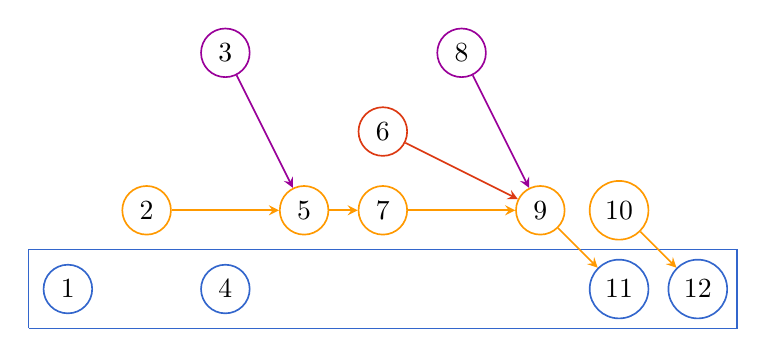
\begin{tikzpicture}[auto, on grid, semithick, state/.style={circle, text=black}]

    \draw[chartblue]
      (-0.5, -0.5) -- (8.5, -0.5) -- (8.5, 0.5) -- (-0.5, 0.5) -- (-0.5, -0.5);

    \node[state, draw=chartblue] (1) {1};
    \node[state, draw=chartyellow, above right= of 1] (2) {2};
    \node[state, draw=chartmagenta, above right= 2cm and 1cm of 2] (3) {3};
    \node[state, draw=chartblue, right= 2cm of 1] (4) {4};
    \node[state, draw=chartyellow, above right=of 4] (5) {5};
    \node[state, draw=chartred, above right=of 5] (6) {6};
    \node[state, draw=chartyellow, right=of 5] (7) {7};
    \node[state, draw=chartmagenta, above right= 2cm and 1cm of 7](8) {8};
    \node[state, draw=chartyellow, right= 2cm of 7] (9) {9};
    \node[state, draw=chartyellow, right=of 9] (10) {10};
    \node[state, draw=chartblue, below right=of 9] (11) {11};
    \node[state, draw=chartblue, below right=of 10] (12) {12};

    \draw (2) edge[chartyellow, -stealth] (5)
          (3) edge[chartmagenta, -stealth](5)
          (5) edge[chartyellow, -stealth] (7)
          (7) edge[chartyellow, -stealth] (9)
          (6) edge[chartred, -stealth] (9)
          (8) edge[chartmagenta, -stealth] (9)
          (9) edge[chartyellow, -stealth] (11)
          (10) edge[chartyellow, -stealth] (12);


  \end{tikzpicture}
  \caption{\mt view of the commits  represented in
    Figure~\ref{fig:repoEvents} showing the path they followed to reach
    the master branch. In this model the successors of each commit
    represents the path followed by that commit to reach the master
    branch.}
  \label{fig:repoTree}
\vspace{-3mm}
\end{figure}

Computing the \mt from a DAG for any repository may not be
possible; however, certain features of the development process of Linux
make it feasible to compute the \mt for the Linux repository.
First, the master branch of Linux is maintained by Linus Torvalds, and
only Linus has write access to it. We have verified this assertion in
previous research~\cite{German2015}. We have developed a heuristic that
is presented in Algorithm~\ref{fig:alg}. In short, the algorithm first
identifies the commits made directly to the master branch; whereafter it
recursively determines the shortest path (in terms of time), using the
DAG, from each commit to the master branch using the inverted DAG.

\begin{algorithm}
        \caption{Computing the \mt from Linux Git's DAG}\label{fig:alg}
        \begin{algorithmic}
                \Function{ComputeMergeTree}{DAG}: tree
                \State {\# Compute the tree from the DAG of Linux repository.}
                \State {\# Returns $Tree$, a graph containing every commit }
                \State {\# in DAG with the path it followed to master.}

                \State $head \gets \textit{Head of master of git repository}$
                \State $master \gets \textit{traverse DAG from head using }$
                \State \quad\quad\quad\quad $\textit{first ancestor until reaching root}$
                \State $nodes(Tree) \gets nodes(DAG)$
                \State \Function{distance2Master}{cid} : seconds
                \State {\# Helper function}
                \State {\# Recursively compute shortest distance to master}
                \State {\# setting cid's successor (next) in its way to master.}
                \State {\# This function should be memoized. Otherwise it}
                \State {\# would run in exponential time.}
                \If {\textit{cid in master}}
                \State \Return 0
                \EndIf
                \State    $d \gets 	\infty$
                \State {\# Traverse the inverted DAG}
                \For{$c \in children(cid, DAG)$}
                \If {$c \in master$}
                \State $d_1 \gets commitTime(c)-commitTime(cid)$
                \Else
                \State {$d_1 \gets distance2Master(c)$}
                \EndIf
                \If {$d_1 < d $}
                \State $next \gets c$
                \State  $d \gets d_1$
                \EndIf
                \EndFor
                \State {\# $c$ is the commit that follows $cid$}
                \State {\# in its way to master}
                \State add edge $(cid, next)$ to $Tree$
                \State \Return $d$
                \EndFunction

                \State {\# Compute the distance for each commit}
                \State {\# discarding result}
                \For{$c \in nodes(DAG)$}
                \State $distance2Master(c)$
                \EndFor
                \State \Return $Tree$
                \EndFunction
        \end{algorithmic}
\end{algorithm}

We evaluate the performance of the heuristic using the merge log made by
Linus Torvalds, the original creator of Linux, and primary merger of all
other repository events into the master branch of the repository. In
Figure~\ref{fig:sampleMerge}, we see an example of the merge log.

\begin{figure}[htbp]
  \centering
  {\fontsize{7}{9}
    \begin{verbatim}
Merge: 8cbd84f fd8aa2c
Author: Linus Torvalds <torvalds@linux-foundation.org>
Date:   Tue Aug 10 15:38:19 2010 -0700

Merge branch 'for-linus' of git://neil.brown.name/md

* 'for-linus' of git://neil.brown.name/md: (24 commits)
md: clean up do_md_stop
[... edited for the sake of space]
md: split out md_rdev_init
md: be more careful setting MD_CHANGE_CLEAN
md/raid5: ensure we create a unique name for kmem_cache...
...
    \end{verbatim}}\vspace{-5mm}
  \caption{Example of how merges record a subset of commits being
    merged. The commit only shows the first 20 one-line summaries
    messages for the 24 non-merge commits it merged. The ending
    ``\ldots'' is part of the log and represents that other
    commits were merged.}
  \label{fig:sampleMerge}
\end{figure}

We use this information to evaluate the accuracy of the \mt model
extracted from the DAG\@. The method we followed started with the
extraction of the commit history up to July 20, 2016. We computed the
merge tree of every commit until then. Since Linus Torvalds mostly does
merging directly into master, we assumed that every merge by him is the
root of a \mt. As described above, the log of a merge-commit usually
contains the number of commits in the merge the first 20 summaries of
commits being merged. We extracted merges by Linus Torvalds using the
command \mycode{log --merges --author='Torvalds} and compared the number
of commits according to the log with the number of commits in the  \mt
rooted in this commit. We also used the summaries of the commits found
in the merge (not necessarily all---see above) to make sure those
commits were in their corresponding merge tree. For example, for the
merge in Figure~\ref{fig:sampleMerge} we would expect that the merge
tree rooted at \mycode{8cbd84f} contains 24 commits, and the one-line
summaries corresponds to commits in that \mt. We also inspected those
with differences to make sure they were true errors.  The results can be
summarized as follows:

\begin{itemize}

  \item

    Five merges were false-errors because their logs did not contain
    accurate information (were probably edited by hand). For example in
    \mycode{42a579a0f\ldots} one commit summary was missing (the line was
    empty), in \mycode {c55d267\ldots} the summaries were reordered.

  \item

    The heuristic correctly identified that 79 of Linus merges (between
    Jun 7, 2014 and Jun 2, 2014) were made to a branch (not master).
    This branch was merged at \mycode{3f17ea6d\ldots} which contained 6809
    commits.

  \item

    The heuristic worked perfectly until Sept 4, 2007, the earliest date
    that it could be verified.  Before this date, and until Dec 12,
    2006, merges did not include a summary of the commits they included,
    hence making it impossible to verify; during this period, however,
    we correctly identified the merges by Linus into master.

  \item

    Before Dec. 12, 2006 (1542 merges) our heuristic breaks due to the
    presence of a \textit{foxtrot} commit (\mycode{c436688\ldots}),
    which confounded the true master branch of a repository (see
    \url{http://bit-booster.blogspot.ca/2016/02/no-foxtrots-allowed.html}
    for a description of the issue).

\end{itemize}

In summary, of the merges after Sept. 4, 2007, our heuristic was correct
in 100\% of the 16,680 commits. It failed in 1,542 commits before Dec.
12, 2006 and in 836 it appears to be correct (Dec 7, 2006 to Sept 4,
2007).

% Evaluation

In order to determine the effectiveness of the merge-tree model on
comprehension and summarization of git repositories, we conducted a
controlled user study on 12 participants. The user study is a
mixed-methods study, with focus on the quantitative aspects in order to
capture how effective the \mt model, if it is, at improving the
correctness, accuracy, and time performance metrics of users when
performing summarization tasks. We use the qualitative questions as a
means of determine the preference of the participants, and what aspects
they preferred from each tool.

We formulate three research questions that this study is attempting to
answer;

\begin{RQ}
  \item

    Is the DAG able to provide users with an understanding of the events
    in a repository?

  \item

    Do \mt make a difference in the ability to summarize basic
    aggregated information?

  \item

    Do users prefer the \mt model to the DAG for summarization and
    comprehension tasks?

\end{RQ}

% Implementation

We implement a tool, \tool, to test and verify the capabilities of the
\mt model. \tool provides search, summarization, and
visualization using the \mt model.

We provide users with search-based navigation. The search engine takes a
plain text query from the user and returns results based on similarity
to the query. The engine weighs various fields, including the commit
log, the author name, the commit hash, and the dates that the commit was
authored and committed. The results are aggregated by the \mt
with a link to the root at the top, and the repository events that match
the search query in a table below.  An example of a single \mt is shown
in Figure~\ref{fig:linvis_search_results}.

\begin{figure}[htpb]
  \centering
  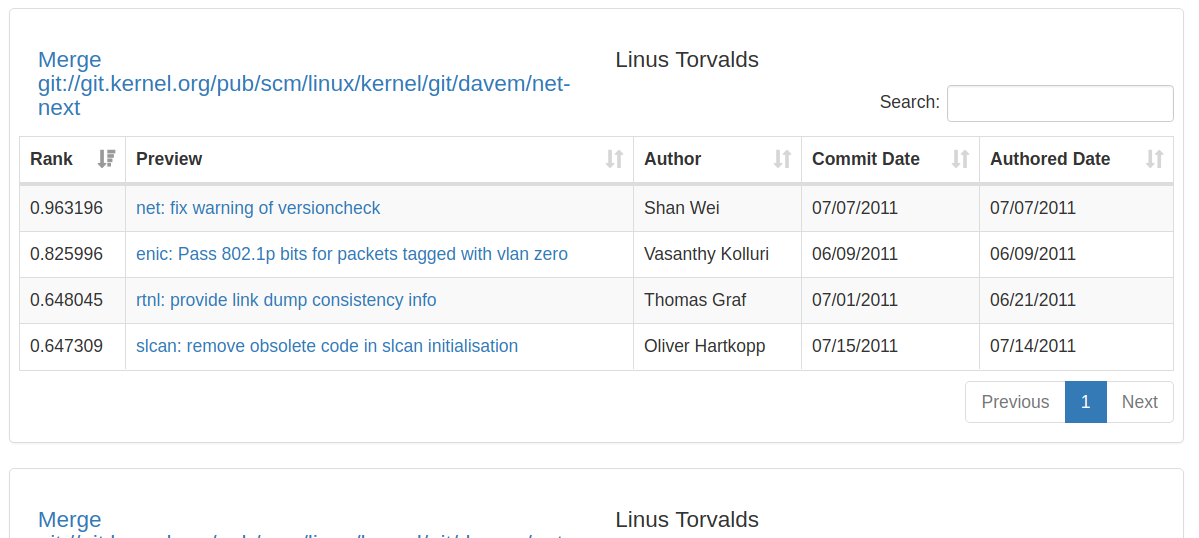
\includegraphics[width=1.0\linewidth]{figures/linvis/search_results.png}
  \caption{\tool search results for `net-next 2011', showing a single
    \mt group.}
  \label{fig:linvis_search_results}
\end{figure}

\tool uses seven tabs to show the information and visualizations for a
selected commit or merge. The message tab shows the full commit log
message. This does not include the diff. The files tab shows an
aggregated table of all files that were modified in a merge. It includes
metrics like the number of lines added, lines removed, total lines
modified, and the delta, summed across all commits in the merge tree
that modify this file. A small details drop-down button allows a user to
see exactly which commit makes the changes, as shown in
Figure~\ref{fig:linvis_files}. If the current repository event being
viewed is a commit, the aggregate views will only show modifications
made by the commit. The modules tab shows the modules modified in the
merge tree. Like the files tab, the modules tab uses a table to show the
name of the module, the number of commits that are in the merge tree
that work with the module, and a details button to provide the links to
those commits.

\begin{figure}[htpb]
  \centering
  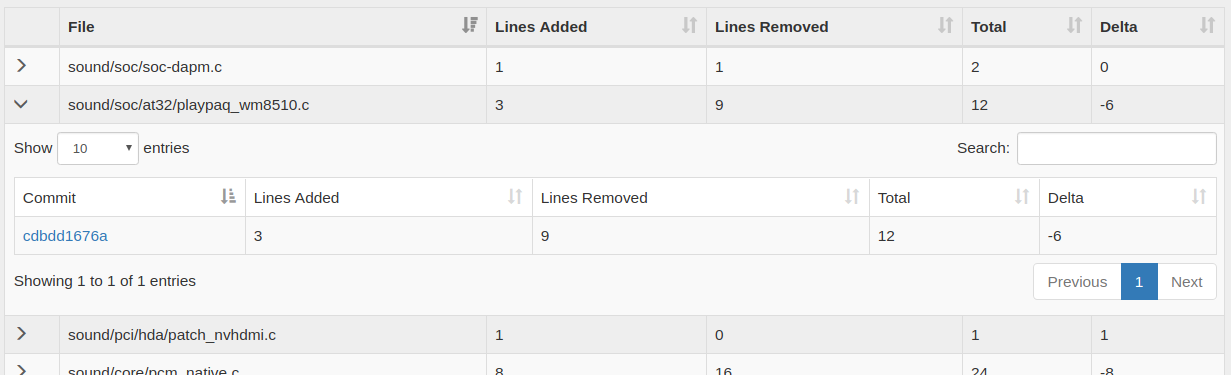
\includegraphics[width=1.0\linewidth]{figures/linvis/linvis_files.png}
  \caption{Table showing the modified files in a merge, with the second
  entry expanded to show the commit that makes the changes.}
  \label{fig:linvis_files}
\end{figure}

The authorship tab is very similar to the files tab, but shows the
authorship information. It shows the sum of the number of lines added,
removed, modified, and the delta within the \mt. It also shows
the number of files that were modified by the author. The details tab is
organized slightly differently. Instead of organizing these results by
commit, the details are organized by file, showing which files were
modified by the author in this \mt (Figure~\ref{fig:linvis_authors}).

\begin{figure}[htpb]
  \centering
  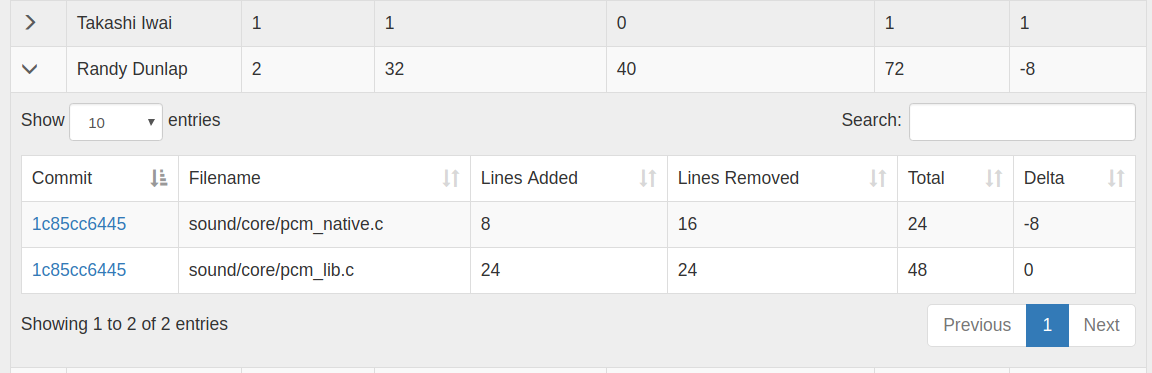
\includegraphics[width=1.0\linewidth]{figures/linvis/linvis_authors.png}
  \caption{Table showing the authors who made changes in a merge. The
    entry for Randy Dunlap is expanded, showing the modifications to
    each file that were made by Randy.}
  \label{fig:linvis_authors}
\end{figure}

\tool implements three visualizations, a list tree, pack tree, and
Reingold-Tilford tree. The list tree is a series of indented textual
lists that can be easily searched with the built-in search in most
web-browsers. The list tree is rooted at the current event, if the event
is a commit, only that commit will be shown; conversely, if the selected
event is the root, the entire merge tree will be shown. The Pack-Tree or
Bubble tree, uses a set-based approach for showing the parent
relationship. The root node aggregates all of the events within the \mt
into the master branch. Thus, the root is the superset of all the other
nodes in the tree. The commits are shown as individual white circles,
containing no other events, as these are the leaves. This is shown in
Figure~\ref{fig:linvis_pack}. The selected event will be shown in bright
orange, commits in white, and merges in shades of blue. Darker shades of
blue indicate that the merge is deeper in the tree.

\begin{figure}[htpb]
  \centering
  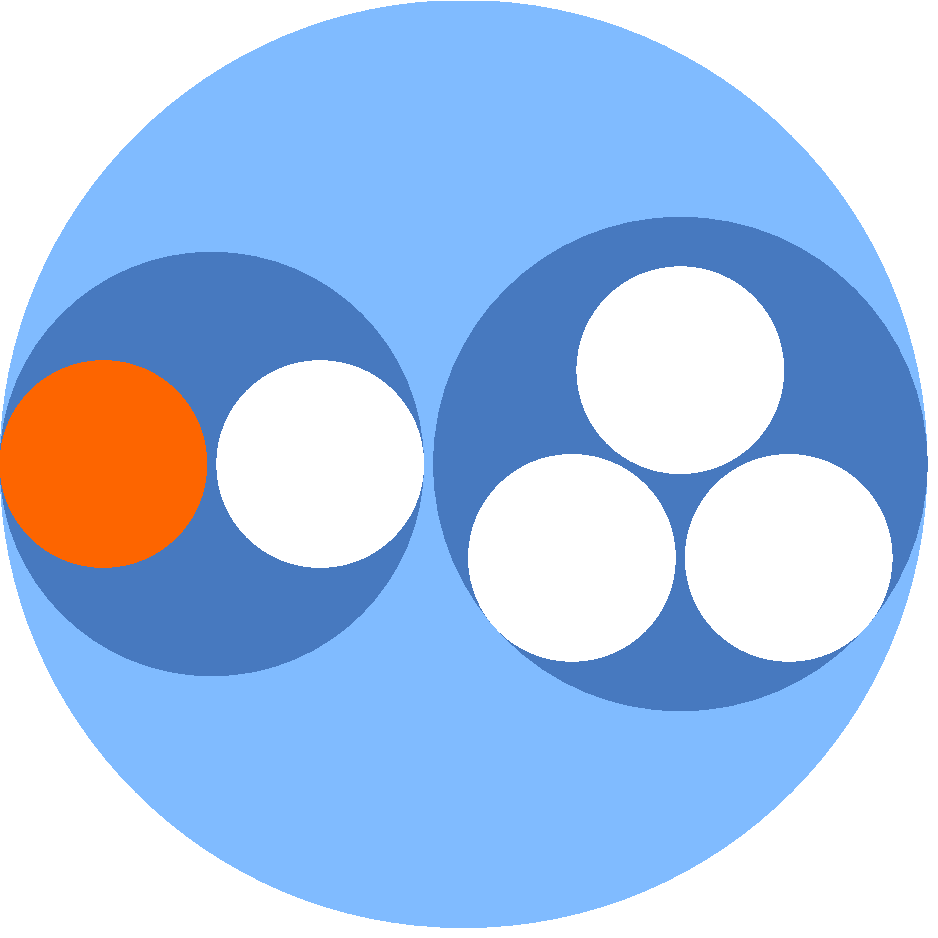
\includegraphics[width=0.8\linewidth]{figures/linvis/linvis_bubble.pdf}
  \caption{The pack tree visualization for a selected commit, shown in
    orange.}
  \label{fig:linvis_pack}
\end{figure}

The Reingold-Tilford tree is the classic tree visualization, with the
root at the top, leaves at the bottom, and the edges between them
showing the parent relationship. An example of the Reingold-Tilford tree
visualization is shown in Figure~\ref{fig:commit_1} and
Figure~\ref{fig:commit_2}.


\section{Related Works}
\label{sec:related_works}

% vim:set et sw=2 ts=4 tw=72:
% Jul 04, 2017
% Evan Wilde

\section{Related Works}
\label{sec:related_works}

Version control systems monitor the development lifetime of software
projects. This makes the version control system vital in providing
information about how a software project is being developed. To do this,
the user must be able to gain a clear understanding of how commits are
being integrated into the project, along with understanding what changes
these commits are bringing with them. These are the tasks that we set
out to solve with the \mt model. Ideally, we could compare our model
against another that is designed with these goals. To our knowledge, we
know of no git repository visualization tool that has these specific
goals. This may be due to issues with finding the master branch of the
repository which is a non-trivial task, or due to other factors. While
we have found no tool with the express goal of showing how a commit is
integrated, and providing a summarization of a merge, there has been a
lot of work done in providing visualizations of various aspects of a
repository.

Many tools work to address the issues in communication between
developers in inter-team collaboration work. Codebook\cite{Begel2010}
uses a data mining technique to determine the developer of a piece of
code, the program manager who wrote the specification for the code, and
the program managers and developers on the team who were working
together. Hipikat\cite{Cubranic2005} is another tool with a focus on
communication. Where Codebook focuses on developers working on a
project, Hipikat is focused on enabling easier integration of new
developers to a project by providing them with easily-searchable
artifacts of the changes made. Codebook is useful for pairing a
contributor with the original developer; however, the developer may not
have worked with the piece of code in years. A Hipikat program may
provide more information to the maintainer as it records the artifacts
of why certain design decisions were made when they were made using
other tools like Bugzilla and CVS.\@ Neither tool is sufficient in
meeting our goals to provide a summary of the topology of the kernel
repository through a visual tree.

Most visualizers provide a visual presentation of a certain aspect of a
repository. Fractal Figures\cite{Ambros2005} uses a unit square to
represent a portion of a project, then partitions the square based on
the proportion of an author's contributions to that portion of the
project. EPOSee\cite{Burch2005} and Evolution Radar\cite{Ambros2009}
perform further analysis, determine which files are made together, and
what changes are made over a sequence of commits, though the goals
behind these projects is different.

Codebook, Hipikat, Fractal Figures, EPOSee, and Evolution Radar all work
with data from CVS repositories. Our goal is to provide information
about Git repositories, specifically the Linux master repository. Fewer
tools are available for generating visualizations and summaries of Git
repositories, potentially due to the DAG model used by Git.

Gource is a tool for providing an interactive timelapse of the state of
a repository\cite{Caudwell2010}. In the timelapse, it shows who
contributes and what type of contribution a developer is making. These
contribution types are one of, adding a file, removing a file, and
changing a file. While the timelapse is interesting to watch, it does
not provide any additional explanation of the changes actually being
made, only the frequency that they are being made and who is making
them. Codeswarm\cite{ogawa09} is similar to Gource, using an organic approach to
visualizing events in the repository. Unlike Gource, which focuses on
the files, Codeswarm focuses on developers and the number of commits
they are making.

Git itself is shipped with summarization and visualization tools: the
\verb|git log| command and Gitk, which is a graphical tool for the
purpose of browsing the DAG of the repository. Many other tools are
designed with a similar visual metaphore as what is presented in Gitk,
including GitKraken, Github Desktop and web interfaces, the Git Lab web
interface, the Bitbucket web interface, are a few examples. The Gitk
interface is built around the central DAG viewer. The DAG displays the
repository events on their respective branches, the author, and the date
that the event was authored. A user can select an event to view addition
information about it, including the full commit log, the parents and
children of the event, and the diff generated if modifications were
made. In the case of the Linux kernel, merges are not resolved as merge
conflicts in the master repository, but by the developers prior to
merging through rebase operations. With this development model, no
merges will have modified any files, and will not show a diff. While the
merge does not make changes directly, the effects of merging the commits
persist, but Gitk is unable to provide an aggregated view of the files
modified, the patches for those files, and the authors who contributed
commits to that merge.

Our tool is primarily aimed at presenting the hierarchical structure of
the Linux git repository. We use tables for presenting the summarized
information of the commits and merges, but this information could also
be presented in a graphical form. Various graphical forms for displaying
file and authorship data exist, the principal forms being matrix views,
city scapes, bar and pie charts, and networks \cite{Eick2002}. Any of
these data visualization metaphors are applicable to our system.

%%% Local Variables:
%%% mode: latex
%%% TeX-master: "lineval.tex"
%%% End:


\section{Controlled User Study}
\label{sec:study}

We use a controlled mixed-methods users study in order to evaluate the
ability for the DAG to provide users with a conceptual image of how a
commit is integrated into a project, to compare the DAG and \mt models,
and determine which model the users preferred.

In this section, we describe the methods used to for designing and
implementing the user study.

\subsection{Questions and Tasks}
\label{sub:questions}

\begin{table*}[htpb]
  \centering
  \caption{Conceptual Tasks }
  \label{tab:conceptual_tasks}
  \begin{tabulary}{0.9\textwidth}{LL}
    \toprule
    Task & Description\\
    \midrule
    T1 & Draw a diagram showing how this commit was merged into the master branch, along with any other related commits\\
    T2 & How many individual commits are related to this commit?\\
    T3 & How many merges are involved with merging this commit into the master branch?\\
    \bottomrule
  \end{tabulary}
\end{table*}

\begin{table}[htpb]
  \centering
  \caption{Summarization Tasks}
  \label{tab:summarization_tasks}
  \begin{tabulary}{\linewidth}{LLL}
    \toprule
    Task Set   & Task & Description\\\midrule
    Merge      & T4   & What is the series of merges involved with merging this
    commit?\\
               & T5   & What other commits are merged?\\
    Authorship & T6   & How many authors are involved?\\
               & T7   & Who contributed the most changes?\\
    Files      & T8   & How many files were modified?\\
               & T9   & Which file had the most changes?\\
    Modules    & T10  & Which modules does this merge tree involve?\\
    \bottomrule
  \end{tabulary}
\end{table}

The questions and tasks are broken down into four groups. The first two
groups are purely quantitative in nature; we begin with conceptual tasks
to understand whether the DAG is capable of providing users with an
understanding of how a commit is merged into the master branch, and
other commits that it is merged with. We continue with summarization
tasks, to quantitatively understand if the \mt model makes a difference
in summarization tasks.

The third task set is purely qualitative, to gain better understanding
of whether participants preferred working with the \mt model in \tool,
or working with the DAG in Gitk, and what aspects they preferred from
each tool. The final group of questions is simply to gain a better
understanding of the demographic of our participants.


\textbf{Conceptual Tasks}




The participants were allowed to use Gitk or the git command line tools
to perform these tasks. These tasks are asked in the specified order,
allowing tabularr to first, create a conceptual understanding of the
commits and merges that will be involved with the rest of the tasks that
follow.tabularmay then use their diagrams to answer T2 and T3. We do not
collect metrics from \tool for the conceptual tasks, opting instead to
determine if the DAG is sufficient for understanding how a commit is
integrated. \tool uses the \mt model show a tree visualization of how
commits are merged, until the commit reaches the master branch.
Table~\ref{tab:conceptual_tasks} shows the conceptual tasks.

We provide the participant with 10 minutes per commit to complete the
first task. The answers to the two other questions in this section are
drawn from the answer in the first task.

\textbf{Summarization Tasks}



The summarization tasks (Table~\ref{tab:summarization_tasks}) are
grouped into task sets by theme. The tasks within the task set are
shuffled, and the task sets are shuffled, to ensure that similar
questions are together, but not in the same order, and to ensure that
the themes are in randomized order between participants. The order of
the commits is shuffled, as well. The order of the tool is randomized,
choosing to start with either \tool or Gitk, to ensure that we do not
place a bias on one tool through the experiment.

As understanding where the merge begins and ends is vital to answering
the other question, the merge task set will always be the first task set
presented; however, the questions will still be re-ordered within the
task set.

\textbf{User Opinion and Profile}

Finally, we ask the user for their opinions on the tools and for some
information about their level of experience with git. This portion of
the study is qualitative and does not rely on either of the tool,
instead attempting to determine which model provided the user with a
better experience.

We do not shuffle the questions in this set of questions, as this should
not have an impact on the opinions of the participant at this point.
These questions are designed to provide us with a better understanding
of preference, and insight on why, the participant had that preference.

We ask the following questions in this order;

\begin{enumerate}
  \item Given these tasks again, which tool would you prefer to use?
  \item Which aspects of each tool did you like and why?
  \item How long have you used git?
  \item If you have used git, for what kind of projects? (personal,
    school courses, professional?)
  \item If you have used git, how many commits, files, and contributors
    were involved with the largest repository you have worked with?
\end{enumerate}

The last three questions in this section are aimed at getting a better
understanding of the demographic of our participants.

\textbf{Procedure}

For each participant, we run a simple python script to generate the
script for the study, eliminating the possibility of bias from us. The
script randomizes the order of the tools, the order of the commits, the
order of the task sets, and the order of the tasks within each task set,
where appropriate.


\subsection{Commit Selection}
\label{sub:commit_selection}

We chose two commits for use in the study. The order that the commits
are presented is randomized between participants, but the order is kept
consistent through the tasks described in the next subsection.

We use the \tool database, containing commits and merge-tree information
from April 16th 2005 to October 14th, 2014, which corresponds to being
between Linux release 2.6.12-rc3 and Linux 3.17-rc1. \evan{Cite the
  database even more?} We chose the commits based on tree sizes. We
found that a majority of the trees contain at most seven inner commits,
while more than 25\% of the trees contain a single commit. 75\% of the
tree contained up to 51 inner commits and merges, and finally the
largest tree contained 7217 nodes. We chose to work with the trees in
the first and second quartile, as merge trees of sizes between one and
seven, not including the merge into the master branch, make up the
majority of the trees in the database.

From here, we selected one tree from the trees of a single commit at
random. Selecting a commit from that tree is trivial, as there is only
one to choose.

We selected one tree of size seven at random from all trees of size
seven. We placed a restriction the trees, the selected tree must include
at least one internal merge to increase the complexity of the trees
tested. After randomly selecting a tree, we chose in internal commit at
random, using the \verb|random.choice| function in python 3.6.1.

Using this technique, we selected commit
\emph{a3c1239eb59c0a907f8be5587d42e950f44543f8} from the tree containing
a single node (Figure~\ref{fig:commit_1}), which we will refer to as
\comA, and commit \emph{cdbdd1676a5379f1d5cbd4d476f5e349f445befe}, from
the tree containing seven nodes (Figure~\ref{fig:commit_2}), which we
will refer to as \comB.

\begin{figure}[bpt]
  \centering
  
\includegraphics[width=0.08\linewidth]{figures/commits/1-commit.pdf}
  \caption{The first merge tree used in the user study, a merge tree
    containing a single commit}
  \label{fig:commit_1}
\end{figure}

\begin{figure}[bpt]
  \centering
  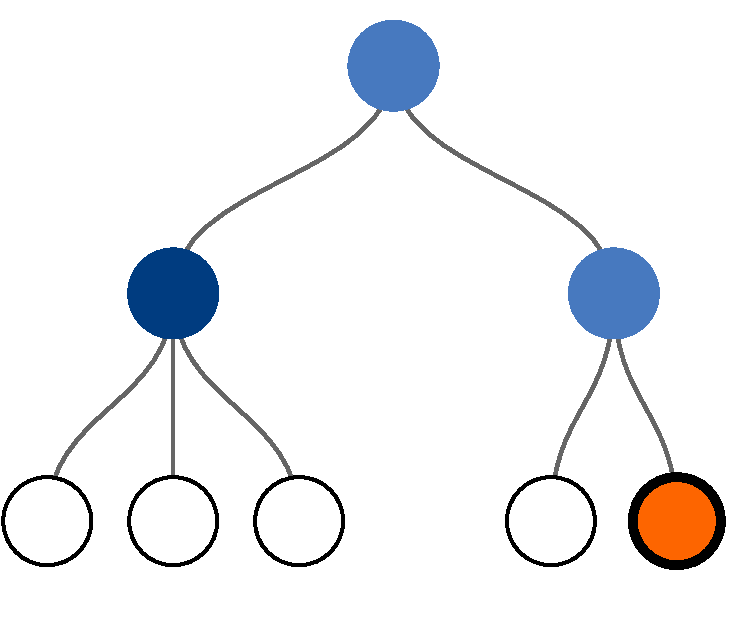
\includegraphics[width=0.5\linewidth]{figures/commits/7-commits.pdf}
  \caption{The second merge tree used in the user study, a merge tree
    containing seven commits}
  \label{fig:commit_2}
\end{figure}



\section{Results}
\label{sec:results}

We recorded the audio and screen capture video for each participant in
the study for further analysis. After capturing the information, we
extracted various metrics from the videos. From the conceptual tasks, we
recorded the time in seconds, and the answer for the question. We
extracted three metrics for the summarization tasks, the time in
seconds, the correctness, and the accuracy. Correctness is a binary
value, it is true if the response was correct and false if the response
was incorrect. The accuracy is measures in distance from the correct
value. An accuracy of zero indicates a correct answer. All tasks in the
summarization tasks include an accuracy metric except T7, which will
only be right or wrong, and therefore cannot meaningfully be measured by
a distance.

\subsection{Conceptual Tasks}
\label{sub:conceptual_tasks}

In Table~\ref{tab:conceptual_results}, we are able to see an overview of
the results from the conceptual questions.


\begin{table*}[htpb]
  \centering
  \caption{Results from the conceptual questions}
  \label{tab:conceptual_results}
  \begin{tabular}{ll|r|lrr|rrr}
    Question                      & Commit & Answer & Median & Mean  & Variance & Median(s) & Mean(s) & Variance(s)\\\hline\hline
    Number of commits in the tree & \comA  & 1      & 4      & 19.11 & 753.11   & 10.0      & 49.92   & 5952.08\\
    Number of merges in the tree  & \comA  & 1      & 5      & 8.27  & 53.62    & 7.5       & 24.67   & 884.42\\\hline
    Number of commits in the tree & \comB  & 5      & 4      & 7.80  & 136.84   & 31.5      & 106.83  & 54123.42\\
    Number of merges in the tree  & \comB  & 3      & 3.5    & 5.40  & 50.27    & 11.0      & 65.6    & 29798.82\\
  \end{tabular}
\end{table*}

Users were able to more closely estimate the number of commits and
merges in the larger tree, but generally took longer than the smaller
tree. The tree with a single node resulted in more variability in the
estimate of number of commits.

It should be noted that these questions were answered after spending
roughly ten minutes attesting to draw a picture that held the answers to
these questions.

\subsection{Summarization Tasks}
\label{sub:summarization_tasks}

In Figure~\ref{fig:summarization_results}, we see all of the
correctness, accuracy, and timing results. The first row of plots are
the correctness results. We see in all cases except for T10, that the
number of instances of a correct result with \tool is roughly the same
as the number of incorrect instances with Gitk. We test each task with
the McNemar Chi-square test~\cite{McNemar1947}.

\begin{figure*}[htpb]
  \centering
  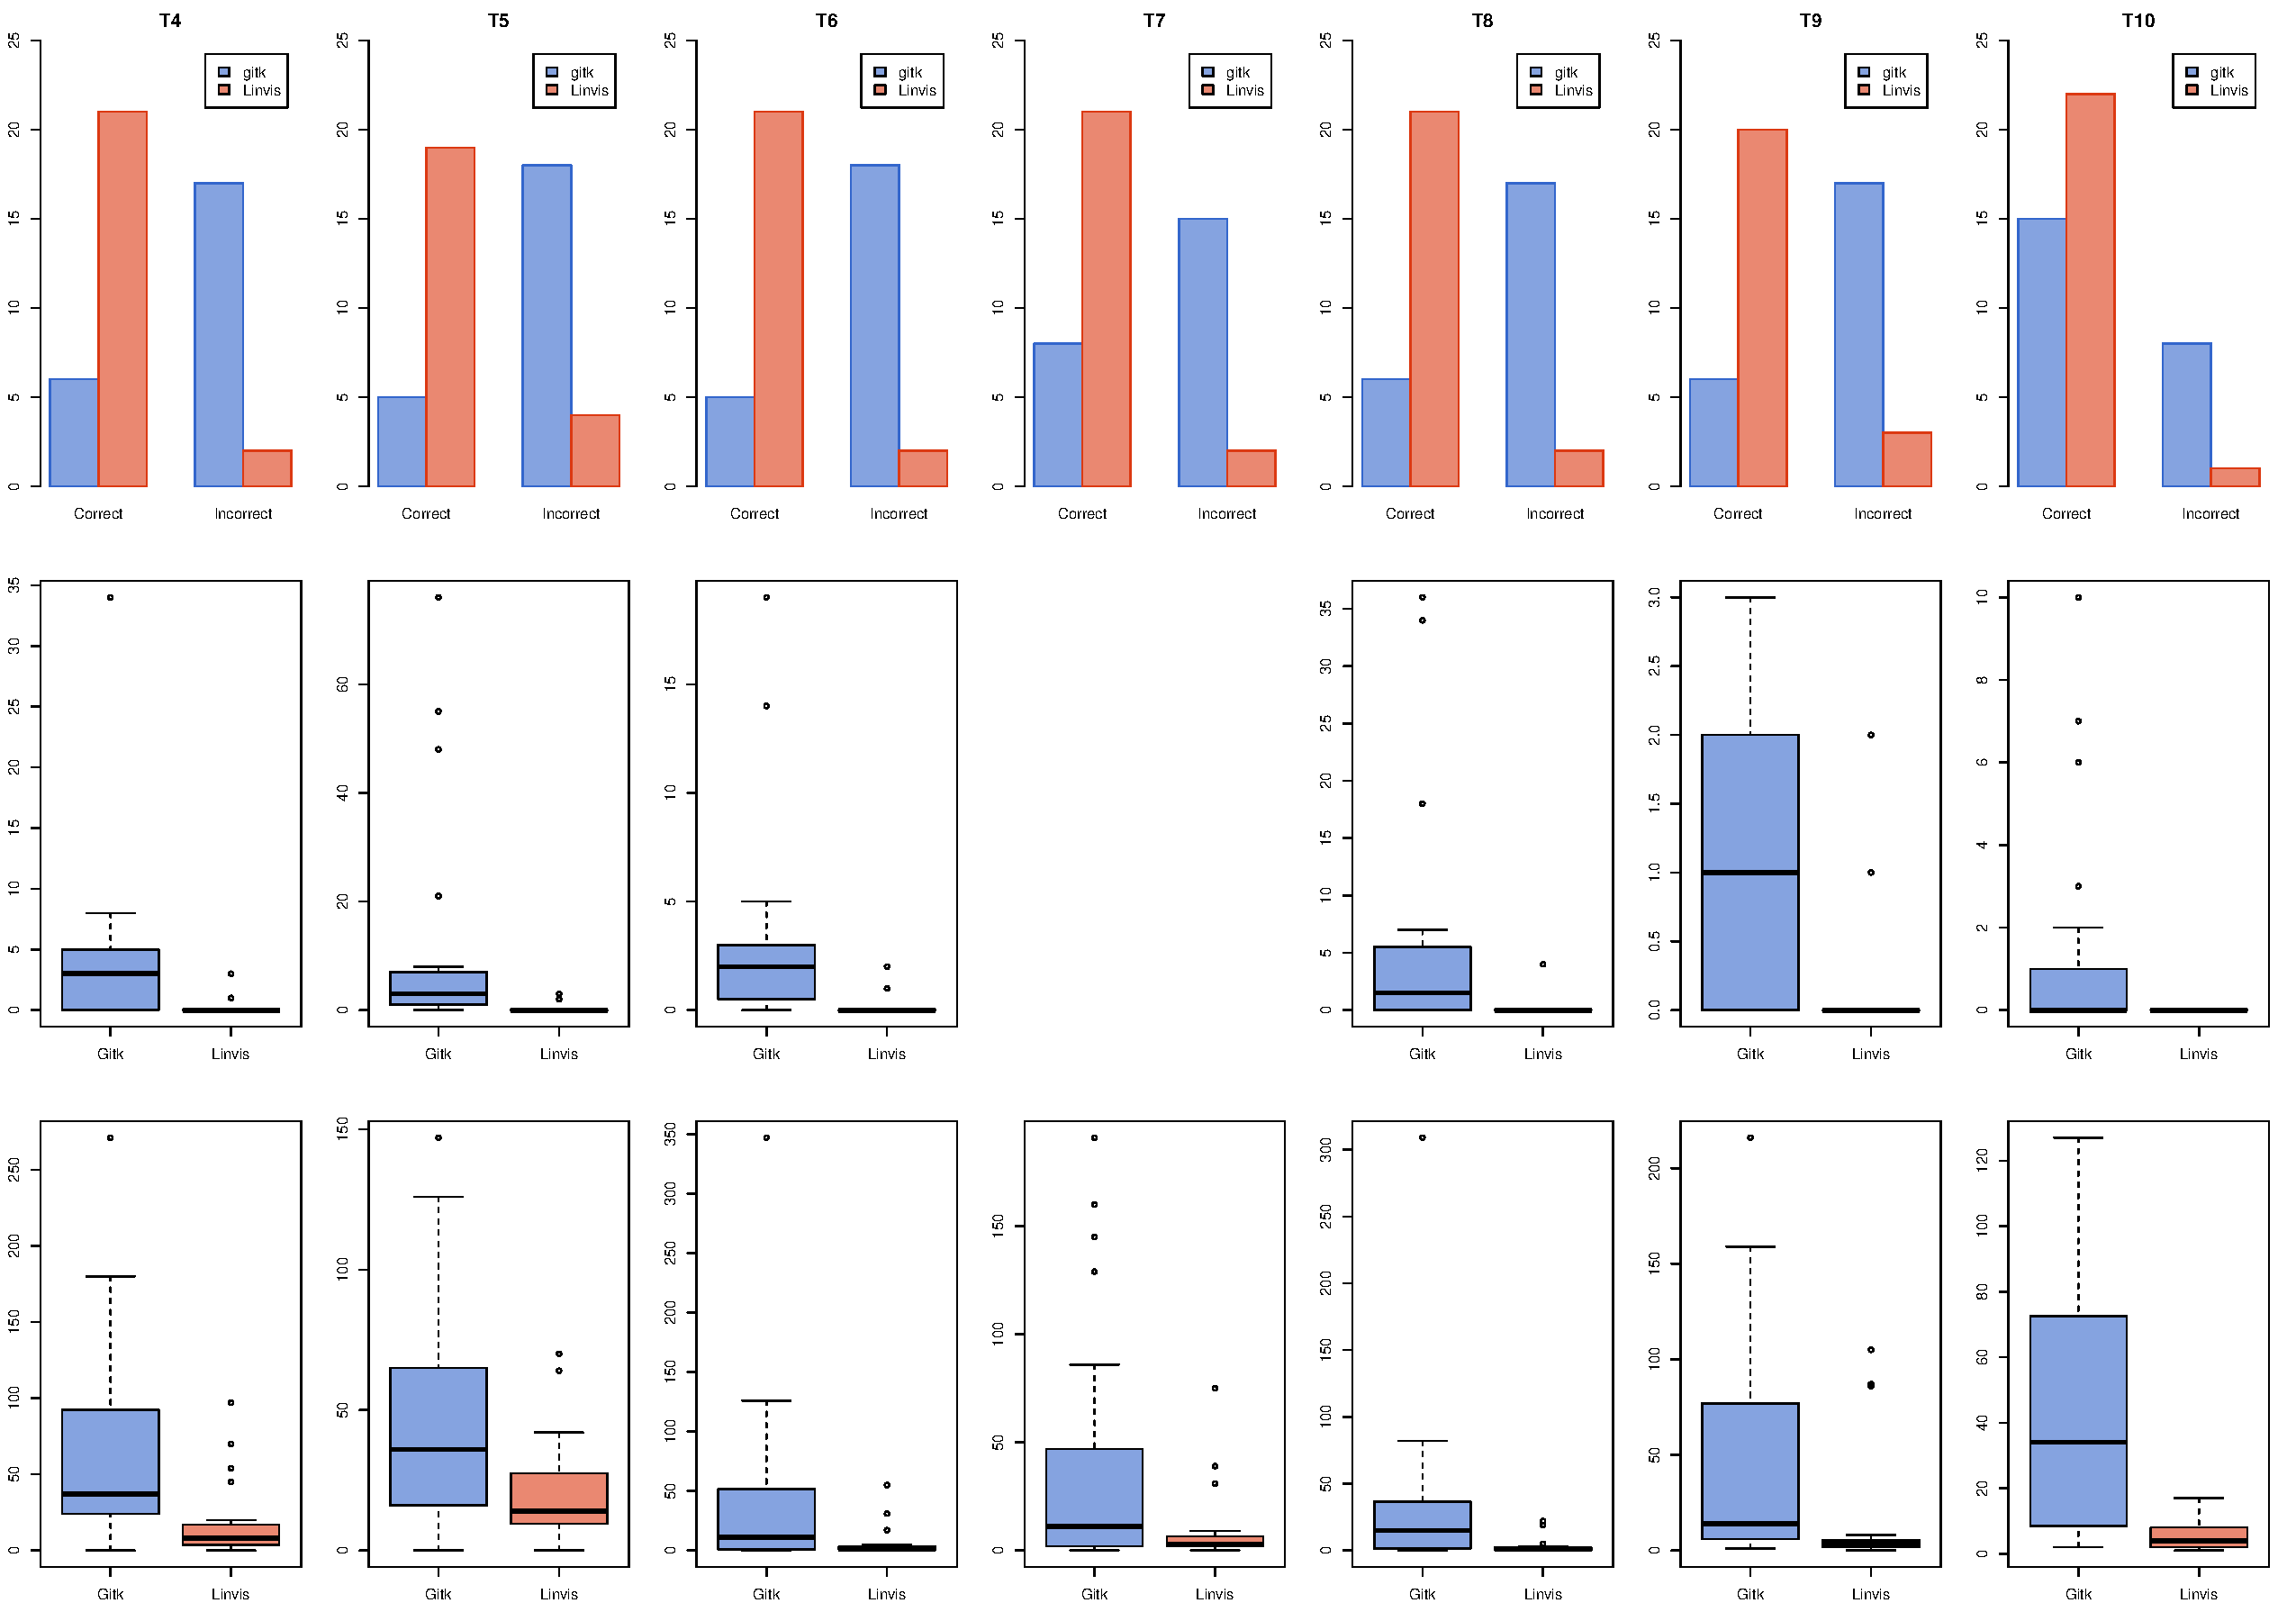
\includegraphics[width=\textwidth]{figures/userstudy/results.pdf}
  \caption{Results from the summarization tasks. The first row plots the
    correctness metric for each task. The second row plots the
    accuracy metric for each task. The third row plots the time metric
    for each task.}
  \label{fig:summarization_results}
\end{figure*}

With the McNemar's tests, we analyze the participants that change from
being correct with one tool to being incorrect with the other. This does
not take into account the number of people who were able to provide the
correct answer for both tools, nor the people who were incorrect for both
tools. The results show whether providing the participants with \tool
over the current standard, gitk, improves the correctness of the
summarization tasks among the participants. We show the results for the
number of people who were, with both tools, correct, incorrect, and
changed in Table~\ref{tab:correctness_table}.

In all cases, except for task T10, we saw statistically significant
results suggesting that we reject the null hypothesis. We tested each
correctness with an $\alpha = 0.005$. The $\chi^2$ test value with one
degree of freedom is $7.879$.

\begin{table*}[htpb]
  \centering
  \caption{Correctness tables showing how many people stayed correct,
    incorrect, and how many people changed between tool}
  \label{tab:correctness_table}
  \begin{tabular}{c|c|c}

    T4 & T5 & T6\\
  \begin{tabular}{cc|rr}
                           &           & \multicolumn{2}{c}{Linvis}\\
                           &           & Correct                      & Incorrect\\\hline
    \multirow{2}{*}{Gitk}  & Correct   & 6                            & 0\\
                           & Incorrect & 15                           & 2\\
  \end{tabular} &

  \begin{tabular}{cc|rr}
                           &           & \multicolumn{2}{c}{Linvis}\\
                           &           & Correct                      & Incorrect\\\hline
    \multirow{2}{*}{Gitk}  & Correct   & 5                            & 0\\
                           & Incorrect & 14                           & 4\\
  \end{tabular}

  &

  \begin{tabular}{cc|rr}
                           &           & \multicolumn{2}{c}{Linvis}\\
                           &           & Correct                      & Incorrect\\\hline
    \multirow{2}{*}{Gitk}  & Correct   & 5                            & 0\\
                           & Incorrect & 16                           & 2\\
  \end{tabular}


  \\\hline
  T7 & T8 & T9\\

  \begin{tabular}{cc|rr}
                           &           & \multicolumn{2}{c}{Linvis}\\
                           &           & Correct                      & Incorrect\\\hline
    \multirow{2}{*}{Gitk}  & Correct   & 8                            & 0\\
                           & Incorrect & 13                           & 2\\
  \end{tabular}  &
  \begin{tabular}{cc|rr}
                           &           & \multicolumn{2}{c}{Linvis}\\
                           &           & Correct                      & Incorrect\\\hline
    \multirow{2}{*}{Gitk}  & Correct   & 6                            & 0\\
                           & Incorrect & 15                           & 2\\
  \end{tabular} &
  \begin{tabular}{cc|rr}
                           &           & \multicolumn{2}{c}{Linvis}\\
                           &           & Correct                      & Incorrect\\\hline
    \multirow{2}{*}{Gitk}  & Correct   & 6                            & 0\\
                           & Incorrect & 14                           & 3\\
  \end{tabular}\\\hline

  & T10 & \\
  & \begin{tabular}{cc|rr}
                            &           & \multicolumn{2}{c}{Linvis}\\
                            &           & Correct                      & Incorrect\\\hline
    \multirow{2}{*}{Gitk}   & Correct   & 14                           & 1\\
                            & Incorrect & 8                            & 0\\
  \end{tabular} & \\

  \end{tabular}
\end{table*}

The correctness test statistics and conclusion for each summarization
task;

The correctness test statistics, conclusions, and a description of the
accuracy and timing results for each summarization task follow:

\begin{itemize}

  \item

    T4; the resulting $\chi^2$ value is $15$. $15 > 7.879$, therefore we
    reject the null hypothesis that \tool does not make a difference in
    the correctness when determining the series of merges that a commit
    takes, with $99.5\%$ confidence.

    There is almost no variation in accuracy between participants using
    \tool, while there is more variance in Gitk. There were two outliers
    among the instances using \tool, which lie within the second and
    third quartiles for the accuracy measure of Gitk. The furthest
    outlier for \tool lies at a distance that is slightly greater than
    the median for Gitk.

    We see similar results in the timing metric; all significant data
    occurs within less time than the second, third, and fourth quartile
    of the Gitk results. Nearly all outlier instances in \tool are
    within the third quartile group of the instances of Gitk with the
    exception of the most extreme, which lies in the fourth quartile
    group.

    The results indicate that \tool is able to assist users with
    determining how a commit is merged more accurately, and more
    quickly.

  \item

    T5; the resulting $\chi^2$ value is $14$. $14 > 7.879$, therefore we
    reject the null hypothesis that \tool does not make a difference in
    the correctness when determining the other related commits, with
    $99.5\%$ confidence.

    There is very little variance in the accuracy of results for \tool
    compared to the accuracy of the results in Gitk. The median distance
    is smaller, indicating that the participants performed more
    accurately using \tool.

    There is less variance in the time taken to come to an answer with
    \tool than with Gitk. Furthermore, we see that a majority of the
    participants were able to complete the task in \tool in much less
    time than 50\% of the participants using Gitk.

    The results indicate that \tool is able to assist users in
    understanding which commits are related to a given commit.

  \item

    T6; the resulting $\chi^2$ value is $16$. $16 > 7.879$, therefore we
    reject the null hypothesis that \tool does not make a difference in
    the correctness when determining the number of authors involved with
    the merge tree, with $99.5\%$ confidence.

    We see the same results from this task as with the previous tasks,
    suggesting that \tool assists users determine the number of authors
    more quickly and more accurately.

  \item

    T7; the resulting $\chi^2$ value is $13$. $13 > 7.879$, therefore we
    reject the null hypothesis that \tool does not make a difference in
    the correctness when determining who contributed the most changes,
    with $99.5\%$ confidence.

    This question does not include an accuracy metric, as there are only
    two possible outcomes. We see the same result in the timing metric
    as we did from the previous questions.

    The results suggest that \tool is able to help users correctly
    identify the person who contributed the most lines of code to a
    merge tree in less time.

  \item

    T8; the resulting $\chi^2$ value is $15$. $15 > 7.879$, therefore we
    reject the null hypothesis that \tool does not make a difference in
    the correctness when determining how many files were contributed,
    with $99.5\%$ confidence.

    The results of this task are the same as in the previous tasks.
    This suggest that \tool is able to assist users determine how many
    files were modified, more quickly and more accurately.

  \item

    T9; the resulting $\chi^2$ value is $14$. $14 > 7.879$, therefore we
    reject the null hypothesis that \tool does not make a difference in
    the correctness when determining which file had the most changes,
    with $99.5\%$ confidence.

    While this question appears to have a similar answer to the correct
    answer for T7, the answer \comA had two files with the same number
    of midifications, thus the participant must correctly identify both
    of these files to be correct. For this reason, we include an
    accuracy metric.

    The results of this task are the same as the previous tasks.
    This suggests that \tool is able to assist users to determine which
    file had the most changes.

  \item

    T10; the resulting $\chi^2$ value is $5.44$. $5.44 < 7.879$,
    therefore we do not reject the null hypothesis, suggesting that
    \tool does not make a difference in determining which modules are
    involved with a merge tree.

    The accuracy and timing results for this task are the same as the
    others, showing that there is less variability in both accuracy and
    the time taken to have an answer between participants using \tool
    than using Gitk. Looking Table~\ref{tab:correctness_table}, we can
    see that, unlike the other questions, a majority of the participants
    were correct using both tools.

\end{itemize}

\subsection{User Opinions}
\label{sub:user_opinions}

Among the 12 pariticipants, there was nearly unanimous agreement that
for conceptual understanding and summarization tasks, \tool was easier
to work with than Gitk. The participants cited the ability to abstract
information about the merge from the clean summarization tables and
simple visualizations. Three participants suggested that someone with a
professional understanding of Gitk and the git commandline may be to
extract the a good conceptual understanding from the DAG, and perform
the summarization tasks from the commandline. One of these three
participants said that they would prefer to have both tools available,
as they are able to complement eachother.

\section{Discussion}
\label{sec:discussion}

\section{Conclusion}
\label{sec:conclusion}

% \nocite{*}

\bibliographystyle{IEEEtran}
\bibliography{references}

\end{document}
